%%%%%%%%%%%%%%%%%%%%% chapter.tex %%%%%%%%%%%%%%%%%%%%%%%%%%%%%%%%%
%
% sample chapter
%
% Use this file as a template for your own input.
%
%%%%%%%%%%%%%%%%%%%%%%%% Springer-Verlag %%%%%%%%%%%%%%%%%%%%%%%%%%

\chapstarthook{The content of this appendix has been submitted to
\emph{XXXXX} [IF2007: 1.144].}

\chapter{Requirements in Web engineering: a systematic literature review.}
\label{a1} % Always give a unique label
% use \chaptermark{}
% to alter or adjust the chapter heading in the running head

\chaptermark{Requirements in Web engineering: a systematic literature review}

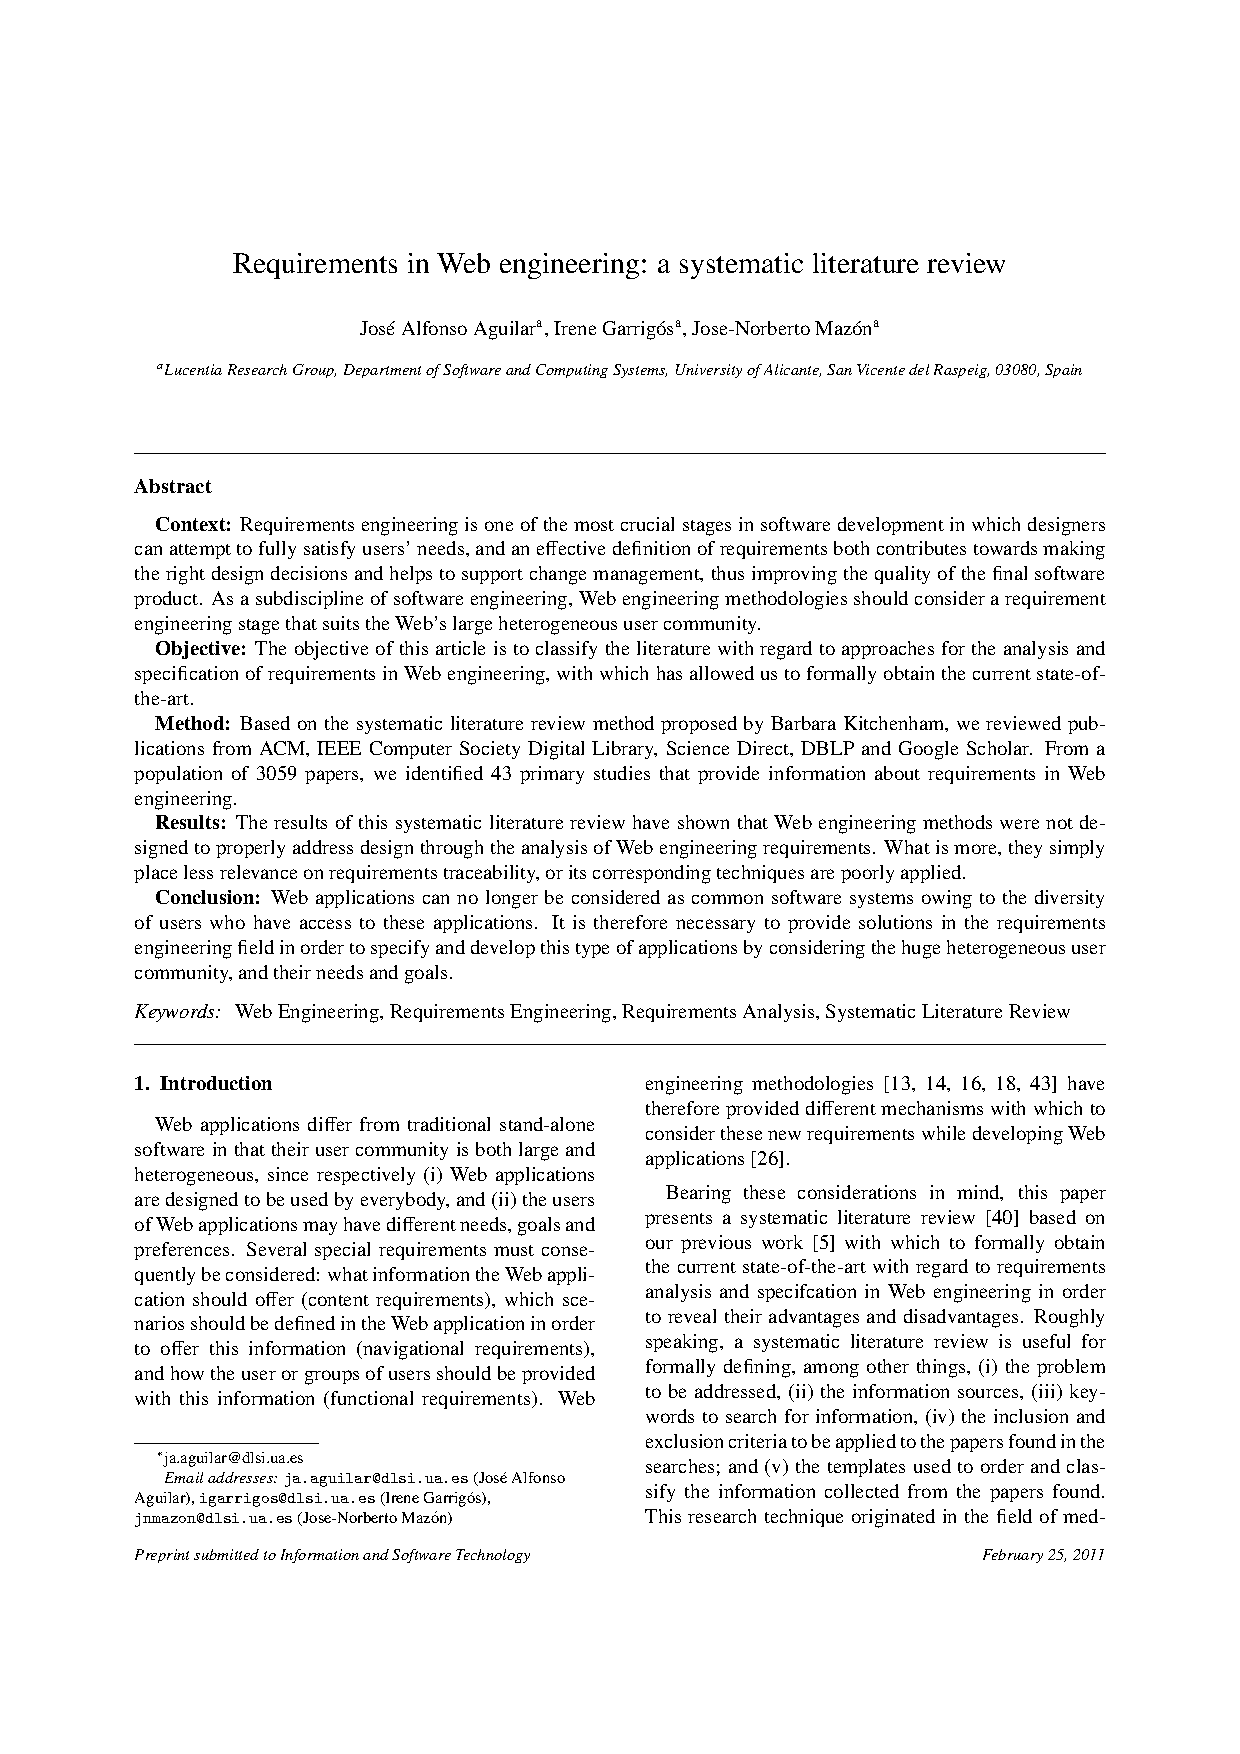
\includepdf[openright=true,pages={1-20}]{papers/apendice/AguilarElsevier2010.pdf}